\documentclass[11pt,a4paper,ngerman]{article}
\usepackage[bottom=2.5cm,top=2.5cm]{geometry} 
\usepackage{babel}
\usepackage[utf8]{inputenc} 
\usepackage[T1]{fontenc} 
\usepackage{ae} 
\usepackage{amssymb} 
\usepackage{amsmath} 
\usepackage{graphicx}
\usepackage{fancyhdr}
\usepackage{fancyref}
\usepackage{listings}
\usepackage{xcolor}
\usepackage{paralist}

%%\usepackage[pdftex, bookmarks=false, pdfstartview={FitH}, linkbordercolor=white]{hyperref}
\usepackage{fancyhdr}
\pagestyle{fancy}
\fancyhead[C]{Höhere Algorithmik}
\fancyhead[L]{Übung Nr. 12}
\fancyhead[R]{WS 2011/12}
\fancyfoot{}
\fancyfoot[L]{}
\fancyfoot[C]{\thepage$\,$ von \pageref{LastPage}}
\renewcommand{\footrulewidth}{0.5pt}
\renewcommand{\headrulewidth}{0.5pt}
\setlength{\parindent}{0pt} 
\setlength{\headheight}{15pt}

\author{Tutor: Lena Schlipf}
\date{}
\title{Max Wisniewski , Alexander Steen}


\usepackage{tikz}
\usetikzlibrary{automata,positioning}


\begin{document}

\lstset{language=Java, basicstyle=\ttfamily\fontsize{10pt}{10pt}\selectfont\upshape, commentstyle=\rmfamily\slshape, keywordstyle=\rmfamily\bfseries, breaklines=true, frame=single, xleftmargin=3mm, xrightmargin=3mm, tabsize=2, mathescape=true}

\maketitle
\thispagestyle{fancy}

%% ----------------------------------
%%		AUFGABE 1
%% ----------------------------------
\subsection*{Aufgabe 1 \mdseries Netzwerkfluss}

Betrachten Sie das folgende Flussnetzwekr $G$.
\begin{center}
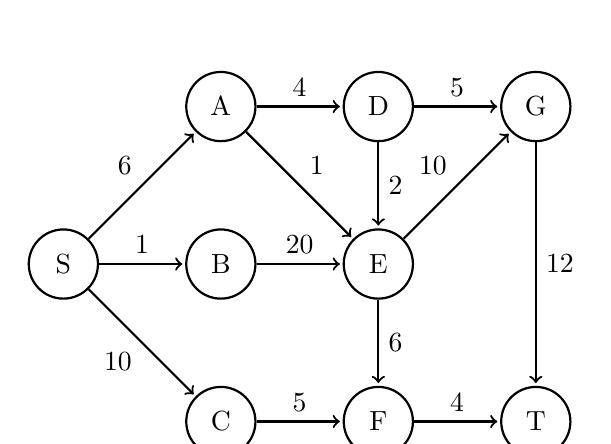
\begin{tikzpicture}[->,shorten >=1pt,node distance=2cm,on grid,auto, thick] 
   \node[state] (S)   {S}; 
   \node[state] (B) [right=of S] {B}; 
   \node[state] (A) [above=of B] {A}; 
   \node[state](C) [below=of B] {C};
   \node[state] (E) [right=of B] {E};
   \node[state] (D) [above=of E] {D};
   \node[state] (F) [below = of E] {F};
   \node[state] (G) [right= of D] {G};
   \node[state] (T) [right = of F] {T};
    \path
    (S) edge  node {6} (A)
          edge  node  {1} (B)
	edge node [swap] {10} (C)
    (A)	edge node {4} (D)
	edge node {1} (E)
    (B)	edge node {20} (E)
    (C)	edge node {5} (F) 
    (D) edge node {2} (E)
	edge node {5} (G)
    (E)	edge node {10} (G)
	edge node {6} (F)
    (F) 	edge node {4} (T)
    (G) edge node {12} (T);
\end{tikzpicture}
\end{center}
Benutzen Sie den Algorithmus von Edmonds und Karp, um einen Maximalen - Fluss von $S$ nach $T$ und einen Minimum-S-T-Schnitt in $G$ zu finden. Zeigen Sie die einzelnen Schritte.\\

\textbf{Lösung:}\\
Wir zeigen die Restgraphen für jede Iteration auf. Dabei wird der Pfad hervorgehoben, der in diesem Schritt gewählt wurde und der mit minimaler Anzahl von Kanten zwischen S und T verläuft.

\begin{center}
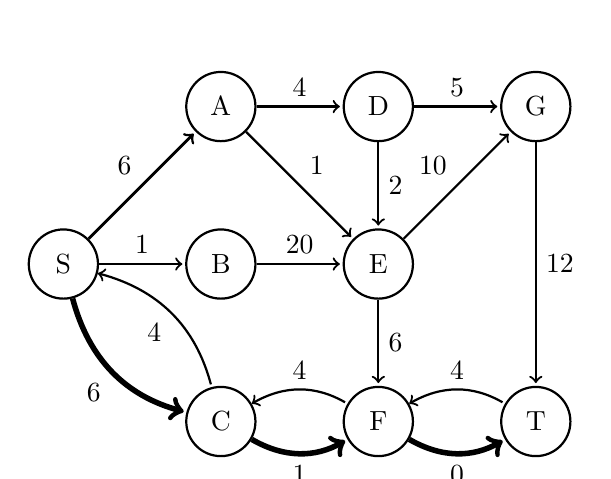
\begin{tikzpicture}[->,shorten >=1pt,node distance=2cm,on grid,auto, thick] 
   \node[state] (S)   {S}; 
   \node[state] (B) [right=of S] {B}; 
   \node[state] (A) [above=of B] {A}; 
   \node[state](C) [below=of B] {C};
   \node[state] (E) [right=of B] {E};
   \node[state] (D) [above=of E] {D};
   \node[state] (F) [below = of E] {F};
   \node[state] (G) [right= of D] {G};
   \node[state] (T) [right = of F] {T};
    \path
    (S) edge[line width = 1pt]  node {6} (A)
          edge  node  {1} (B)
	edge [line width = 2pt, bend right] node [swap] {6} (C)
	edge [<-, bend left]  node[swap] {4} (C)
    (A)	edge node {4} (D)
	edge node {1} (E)
    (B)	edge node {20} (E)
    (C)	edge [line width = 2pt, bend right] node [swap] {1} (F) 
    	edge [<-,bend left] node {4} (F) 
    (D) edge node {2} (E)
	edge node {5} (G)
    (E)	edge node {10} (G)
	edge node {6} (F)
    (F) 	edge [line width=2pt, bend right] node [swap] {0} (T)
	edge [<-, bend left] node {4} (T)
    (G) edge node {12} (T);
\end{tikzpicture}


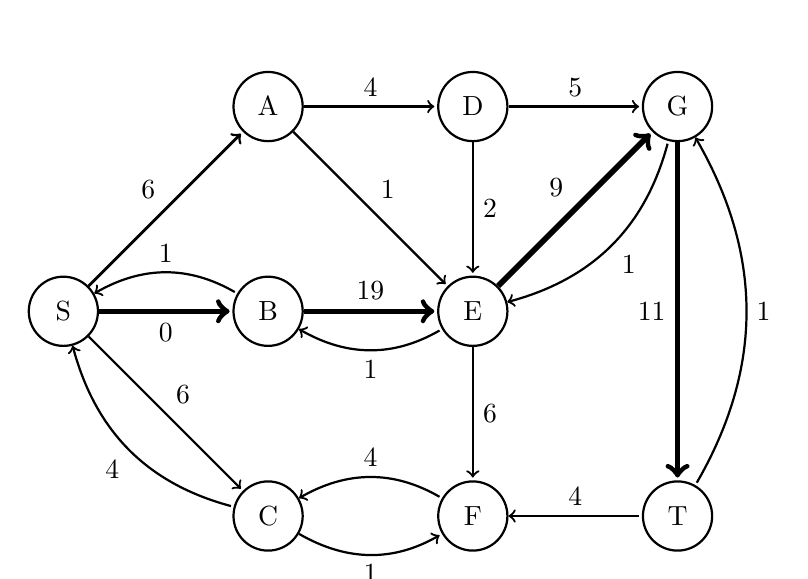
\begin{tikzpicture}[->,shorten >=1pt,node distance=2.6cm,on grid,auto, thick] 
   \node[state] (S)   {S}; 
   \node[state] (B) [right=of S] {B}; 
   \node[state] (A) [above=of B] {A}; 
   \node[state](C) [below=of B] {C};
   \node[state] (E) [right=of B] {E};
   \node[state] (D) [above=of E] {D};
   \node[state] (F) [below = of E] {F};
   \node[state] (G) [right= of D] {G};
   \node[state] (T) [right = of F] {T};
    \path
    (S) edge[line width = 1pt]  node {6} (A)
          edge [<-,bend left]  node {1} (B)
	edge [line width = 2pt] node [swap] {0} (B)
	edge  node {6} (C)
	edge [<-, bend right]  node[swap] {4} (C)
    (A)	edge node {4} (D)
	edge node {1} (E)
    (B)	edge [line width = 2pt] node {19} (E)
	edge [<-, bend right] node [swap] {1} (E)
    (C)	edge [bend right] node [swap] {1} (F) 
    	edge [<-,bend left] node {4} (F) 
    (D) edge node {2} (E)
	edge node {5} (G)
    (E)	edge [line width = 2pt] node {9} (G)
	edge [<-, bend right] node[swap] {1} (G)
	edge node {6} (F)
    (F)  edge [<-] node {4} (T)
    (G) edge [line width = 2pt] node [swap] {11} (T)
	edge[<-, bend left] node {1} (T);
\end{tikzpicture}



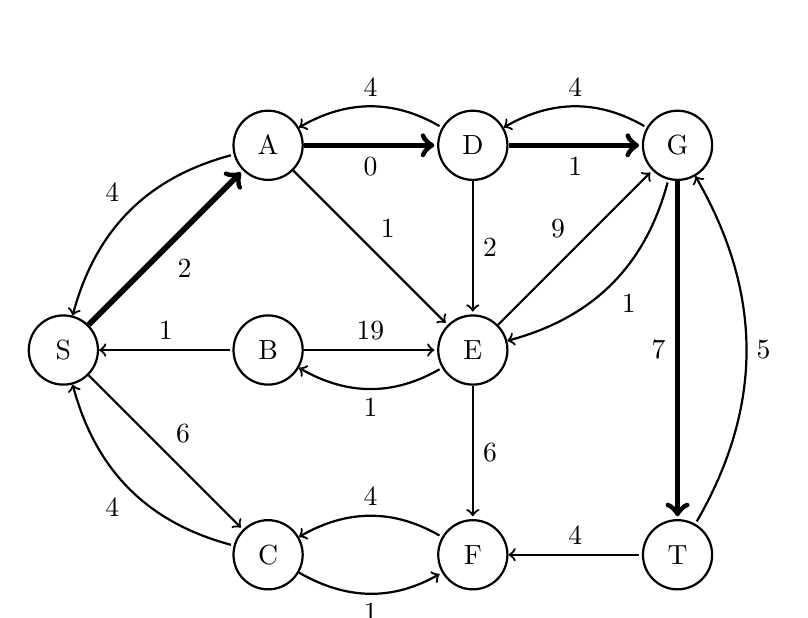
\begin{tikzpicture}[->,shorten >=1pt,node distance=2.6cm,on grid,auto, thick] 
   \node[state] (S)   {S}; 
   \node[state] (B) [right=of S] {B}; 
   \node[state] (A) [above=of B] {A}; 
   \node[state](C) [below=of B] {C};
   \node[state] (E) [right=of B] {E};
   \node[state] (D) [above=of E] {D};
   \node[state] (F) [below = of E] {F};
   \node[state] (G) [right= of D] {G};
   \node[state] (T) [right = of F] {T};
    \path
    (S) edge[line width = 2pt]  node [swap] {2} (A)
	edge [<-, bend left] node {4} (A)
          edge [<-]  node {1} (B)
	edge  node {6} (C)
	edge [<-, bend right]  node[swap] {4} (C)
    (A)	edge [line width = 2pt] node [swap] {0} (D)
	edge [<-, bend left] node {4} (D)
	edge node {1} (E)
    (B)	edge  node {19} (E)
	edge [<-, bend right] node [swap] {1} (E)
    (C)	edge [bend right] node [swap] {1} (F) 
    	edge [<-,bend left] node {4} (F) 
    (D) edge node {2} (E)
	edge [line width = 2pt] node [swap] {1} (G)
	edge [<-, bend left] node {4} (G)
    (E)	edge  node {9} (G)
	edge [<-, bend right] node [swap] {1} (G)
	edge node {6} (F)
    (F)  edge [<-] node {4} (T)
    (G) edge [line width = 2pt] node [swap] {7} (T)
	edge[<-, bend left] node {5} (T);
\end{tikzpicture}


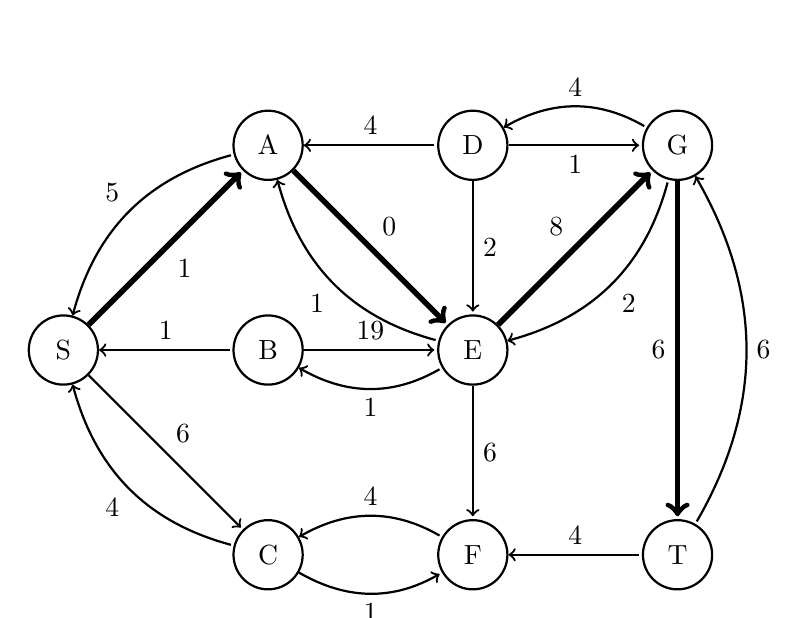
\begin{tikzpicture}[->,shorten >=1pt,node distance=2.6cm,on grid,auto, thick] 
   \node[state] (S)   {S}; 
   \node[state] (B) [right=of S] {B}; 
   \node[state] (A) [above=of B] {A}; 
   \node[state](C) [below=of B] {C};
   \node[state] (E) [right=of B] {E};
   \node[state] (D) [above=of E] {D};
   \node[state] (F) [below = of E] {F};
   \node[state] (G) [right= of D] {G};
   \node[state] (T) [right = of F] {T};
    \path
    (S) edge[line width = 2pt]  node [swap] {1} (A)
	edge [<-, bend left] node {5} (A)
          edge [<-]  node {1} (B)
	edge  node {6} (C)
	edge [<-, bend right]  node[swap] {4} (C)
    (A)	edge [<-] node {4} (D)
	edge [line width = 2pt] node {0} (E)
	edge [<-, bend right] node [swap] {1} (E)
    (B)	edge  node {19} (E)
	edge [<-, bend right] node [swap] {1} (E)
    (C)	edge [bend right] node [swap] {1} (F) 
    	edge [<-,bend left] node {4} (F) 
    (D) edge node {2} (E)
	edge node [swap] {1} (G)
	edge [<-, bend left] node {4} (G)
    (E)	edge [line width = 2pt] node {8} (G)
	edge [<-, bend right] node [swap] {2} (G)
	edge node {6} (F)
    (F)  edge [<-] node {4} (T)
    (G) edge [line width = 2pt] node [swap] {6} (T)
	edge[<-, bend left] node {6} (T);
\end{tikzpicture}

\end{center}

An dieser Stelle sind wir fertig. Wir sehen, dass es keinen Pfad von S nach T gibt. Der Algorithmus bricht ab. Wir können nun den Schnitt konstruieren, indem wir die Knoten zerlegen in diejenigen, die wir von S aus erreichen und die, die wir von S aus nicht erreichen in unserem Restgraphen.\\

Der Schnitt ist also $S=(A,B)$, mit $A=\{ S, A, C, F\}$ und $B=\{ B, E, D,  G, T \}$. Den Fluss können wir bestimmen, indem wir uns ansehen, wie viel aus S rausfließt. Dies steht für uns an den Kanten, die in S reinfließen, da diese zu Beginn nicht existierten. Der Fluss ist in unserem Fall 10.
%% ----------------------------------
%%		AUFGABE 2
%% ----------------------------------
\subsection*{Aufgabe 2 \mdseries Flüsse, Paarungen, Knotenüberdeckungen}

\begin{enumerate}[\bfseries a)]


%% ----------------------------------
%%			a)
%% ----------------------------------
\item Sei $G$ ein Flussnetzwerk, in dem alle Kapazitäten ganzzahlig sind. Beweisen Sie: Es existiert ein Maximum-Fluss $f^*$ für $G$, der nur ganzzahlige Werte annimmt. Zeigen Sie auch, dass man $f^*$ in Polynomialzeit berechnen kann.\\

\textbf{Lösung:}\\

Wir verwenden den Algorithmus von Edmunds-Karp, da dieser auf reellen Kantengewichtet. Dies bedeutet insebsondere, dass er mit $\mathbb{Z} \subset \mathbb{R}$ eine Lösung liefert. Diese liegt nun insbesondere ersteinmal in $\mathbb{R}$. Betrachten wir aber nun, dass die Operationen in Edmunds Karp zur Bestimmung des Flusses nur $+$, $-$, $min$ ist, dann ist zu Beobachten, dass dies Operationen in $\mathbb{Z}$ abgeschlossen sind. Damit ist der resutlierende Fluss auch in $\mathbb{Z}$.\\

Da wir nun Edmunds-Karp verwenden können um das Problem zu lösen, wissen wir nach der Vorlesung, dass dieser eine Laufzeit von $O(|V|\cdot |E|^2)$ hat und damit polynomiell ist.

%% ----------------------------------
%%			b)
%% ----------------------------------
\item Sei $H= \left( V , E \right)$ ein ungerichteter bipartiter Graph. Eine \emph{Paarung} in $H$ ist eine Menge $M \subseteq E$, so dass keine zwei Kanten in $M$ einen gemeinsamen Endpunkt haben. Geben Sie einen effizienten Algorithmus an der eine größtmögliche Paarung in $H$ bestimmt. Was ist die Laufzeit?\\

\textbf{Lösung:}

Wir nehmen bei dem bipartiten Graphen an, dass $V = A \cup B$ und $A \cap B = \emptyset$ die Partition der Knotenmenge ist.

Wir konstruieren einen Graphen $H' = (V', E')$ in der Art, dass $V' = V \cup \{ S, T \}$ zwei neue Knoten, in der Art, dass diese beiden Knoten noch nicht drin sind und im Algorithmus unsere Source und unser Target sind. \\
$V' = \{ (v,w) \; | \; \{v,w\} \in E \, \land \, v \in A \, \land \, w \in B\} \cup \{ (S,v) \;| \; v \in A\} \cup \{ (v,T) \; | \; v \in B \}$.\\
Die Kosten jeder Kante soll $1$ sein. Unsere Kapazitätsfunktion ist also eine konstante $1$ Funktion.\\


\textbf{Satz:} Edmunds-Karp Algorithmus liefert eine größtmögliche Paarung von $H$, indem man von $H'$ alle des Flusses nimmt (wieder mit den ungerichteten aus $H$ identifiziert), die danach ursprünglich in $H$ lagen.\\

\textbf{Beweis:}\\
 \textbf{Teil 1:} Die Lösung bildet eine Paarung.\\

Wir beobachten, dass in jedem Knoten aus $A$ nur ein Fluss von $1$ austreten kann, da nur eine Kante von $S$ auf diesen Knoten führt mit einem Gewicht von $1$. Wir haben keine Kanten von $B$ nach $A$ und keine Kanten in $A$. Das heißt der größte Fluss aus diesem Knoten ist 1. Da Edmunds-Karp wie in a) gezeigt immer nur ganze Gewichte vergibt, wird maximal eine Kante von einem Knoten aus $A$ ausgehen.\\
Analog führt aus $B$ nur eine Kante raus nach $T$, keine Kanten laufen innerhalb von $B$ und es läuft nach konstruktion keine Kante zurück nach $A$. Es wird also maximal eine Kante auf diesen Knoten in $B$ zulaufen.\\

Wir haben also gezeigt, dass die Kanten, die der Fluss nimmt, und zwischen der Partition entlang verliefen, maximal eine Kante einen jeden Knoten in $H$ berühren kann.\\

\textbf{Teil 2:} Die Lösung ist maximal.\\

Hier nutzen wir die Eigenschaft von Edmunds-Karp aus, dass der Fluss maximal ist. Da wir jede Kante mit einem Gewicht von 1 versehen haben, ist der maximale Fluss gleich der Anzahl von Kanten, die unsere Paarung bilden. Da wir nun aber den maximalen Fluss gefunden haben, nachdem wir den Algorithmus ausgeführt haben, haben wir auch eine maximale Anzahl von Kanten, die von $A$ nach $B$ verlaufen können.\\

Sollten wir eine Kante mehr finden, die eine Paarung bilden kann, dann hätten wir dementsrpechend diese neue Paarung als Fluss wählen können und so wäre der Fluss nicht maximal.\\

Die Laufzeit lässt sich nach oben durch die Laufzeit von Edmunds - Karp abschätzen. Der Algorithmus wird auf jedenfall nicht langsamer laufen als $O( |V| \cdot |E|^2 )$, aber es wäre möglich, dass die spezielle Konfiguration ihn schneller macht.

%% ----------------------------------
%%			c)
%% ----------------------------------
\item $H = \left( V, E \right)$ ein ungerichteter bipartiter Graph. Eine \emph{Knotenüberdeckung} für $H$ ist eine Menge $C \subseteq V$ von Knoten, so dass jede Kante $e \in E$ zu mindestens einem Knoten in $C$ inzident ist. Geben Sie einen effizienten Algorithmus an, der eine kleinstmögliche Knotenüberdeckung für $H$ findet.\\

\textbf{Lösung:}\\

Wir haben uns den Satz von König angesehen, aber keine Lust mehr empfunden, diesen umzuformulieren.


\end{enumerate}

%% ----------------------------------
%%		AUFGABE 3
%% ----------------------------------
\subsection*{Aufgabe 3 \mdseries Kantenzusammenhang}

Der \emph{Kantenzusammenhang } eines ungerichteten Graphen $G = (V , E)$ ist die kleinste Zahl $K$ an Kanten, die entfernt werden müssen, damit $G$ unzusammenhängend ist.\\

Zeigen Sie, dass man den Kantenzusammenhang von $G$ durch Berechnung der maximalen Flüsse in höchstens $|V|$ Netzen mit jeweils $O(|V|)$ Knoten und $O(|E|)$ Kanten bestimmen kann.\\

\textbf{Lösung:}\\

Als erstes zeigen wir, wie man mit $|V|^2$ vielen Netzen den Zusammenhang berechnen kann, um dann die Lösung so zu reduzieren, dass man nur noch $|V|$ viele Netze braucht.\\

Ein jedes dieser Netze konstruieren wir wie folgt:\\
Wir behalten alle Knoten unseres Graphen und für die ungerichteten Kanten, konstruieren wir einfach 2 Kanten, eine in jede Richtung. Die Gewichte setzen wir nun für jede Kante auf 1.\\

Nun bauen wir die Netze, dass wir alle Kombinationen $s\in V$ und $t \in V \setminus{s}$ nehmen und den maximalen Fluss s-t im Graphen berechnen.\\

Ein Schnitt in diesem Graphen ist nun eine Partition in 2 Komponente und der Fluss ist die Anzahl der Kanten (da jede Kante Gewicht 1 hat), die über diesen Schnitt gehen. Da die Menge Partitioniert ist und wir alle Kanten gezählt haben, wissen wir, dass wenn wir diese Kanten entfernen, dann bricht der Graph auseinander. Da der Schnitt minimal ist, wissen wir, dass es auf dem Weg, den wir gewählt haben keine geringeren Verbindungen geben kann.

Wenn wir dies nun für alle Kombinationen berechnet haben und davon nun das Minimum nehmen, dann haben wir damit den Kantenzusammenhang bestimmt.

\textbf{Beweis:} Der Algorithmus liefert genau den Kantenzusammenhang.\\

$>$:\\
Angenommen der Algorithmus würde einen größeren Wert (a) liefern als der Kantenzusammenhang (k) ist. Dann existiert ein Schnitt der k Kanten durchtrennt und den Graphen damit in 2 Teile partitioniert. Nun wissen wir aber, dass in unserem Netz maximal $k$ Fluss über den Schnitt fließen kann. Da nicht mehr über den Schnitt kann, kann auch unser gesamter Fluss nicht größer sein. Damit haben wir einen Wiederspruch.\\

$<$:\\
Angenommen der Algorithmus würde einen kleineren Wert (a) liefern als der Kantenzusammenhang (k) des Graphen ist.\\
Dann würde das bedeuten, dass wir einen minimalen Schnitt gefunden haben, über den a Kanten gehen und wenn man diese Weg nimmt, dann würde der Graph in 2 Komponenten zerfallen. Damit kann der Kantenzusammenhang nicht $k>a$ gewesen sein.\

Damit muss der Algorithmus den Korrekten Kantenzusammenhang liefern.\\

\textbf{Optimierung:}\\
Wenn man sich diesen Algorithmus einmal anguckt, dann sehen wir als aller erstes, dass die Schnitt und Flüsse, die uns s und t liefern abelsch sind. D.h. es ist egal ob wir s-t Flüsse berechnen oder t-s Flüsse. Dies ist natürlich so, da unser Fluss ja ungerichtet ist.\\

Nun kann man sich als nächstes Überlegen, dass wenn wir uns einmal 3 Knoten (a,b,v) betrachten und zwischen diesen Paarweise die Flüsse berechnen, ein Fluss zwischen 2 Knoten (o.B.d.A. a und b) nicht kleiner sein kann, als die ein Fluss von min { a-> c, c -> b}. Wir erfüllen also die Dreiecksungleichung. Damit können wir den Algorithmus beschleunigen.\\

Wir müssen also absofort nicht mehr die Startknoten verschieben, sondern nur noch die Zielknoten.\\
Wir brauchen also nur noch $|V|-1$ Netze und können darüber, wie oben gezeigt, trotzdem noch den korrekten Minimalen Schnitt berechnen. Insgesammt haben wir auch nur $|V| = O(|V|)$ Knoten und $2|E| = O(|E|)$ Kanten benötigt.\\

Damit haben wir einen Algorithmus, der diese Spezifikationen erfüllt. 

\label{LastPage}
\end{document}
